\section*{Bài tập 05 --- Similarity-based learning}

Quy ước khoảng cách Euclidean giữa hai vector \(\mathbf{u},\mathbf{v}\) là
\(\|\mathbf{u}-\mathbf{v}\|_2\). Với dữ liệu nhị phân, khoảng cách Hamming là
\(\sum_i |u_i-v_i|\).

%--------------------------------------------------------------------
\subsection*{Câu 1. k-NN cơ bản}

Vector thử \(\mathbf{x}=(6{,}5,\,55,\,5)\). Tính căn của tổng bình phương sai lệch theo từng chiều (GPA, điểm bài tập, điểm project); sắp xếp tăng theo $d$:

\begin{center}
{\small
\begin{tabular}{@{}crrrr@{}}\toprule
STT & GPA & Assign & Proj & $d$ \\\midrule
6 & 6,2 & 50 & 5 & $5{,}009$ \\
3 & 6,0 & 45 & 5 & $10{,}012$ \\
4 & 5,5 & 40 & 4 & $15{,}067$ \\
5 & 7,8 & 70 & 7 & $15{,}188$ \\
2 & 8,2 & 75 & 8 & $20{,}295$ \\
1 & 9,0 & 88 & 9 & $33{,}335$ \\\bottomrule
\end{tabular}
}
\end{center}

\textbf{$k=3$:} ba láng giềng gần nhất là mẫu 6, 3, 4 --- cùng nhãn \textbf{Fail}. Đa số: \textbf{Fail}.

\textbf{$k=1$:} láng giềng mẫu 6 ($\approx 5{,}009$) $\Rightarrow$ \textbf{Fail}.

\textbf{$k=5$:} thêm mẫu 5 (\textbf{Pass}) và 2 (\textbf{Pass}) nhưng vẫn có ba \textbf{Fail} trong năm láng giềng đầu tiên không đổi kết luận đa số: năm láng giềng gần nhất gồm 6,3,4,5,2 --- \textbf{Fail} vẫn chiếm đa số (3 so với 2). Dự đoán: \textbf{Fail}.

\textit{Nhận xét:} Với mẫu thử nằm gần cụm điểm GPA thấp / bài tập thấp, $k$ nhỏ và $k$ trung bình đều giữ nhãn \textbf{Fail}. Chỉ khi $k$ đủ lớn để kéo thêm nhiều điểm \textbf{Pass} xa hơn mới có thể đổi lớp (ở đây $k=5$ vẫn chưa đổi).

%--------------------------------------------------------------------
\subsection*{Câu 2. k-NN và Min--Max}

Dùng $k=3$ như mặc định bài tập (đề không ghi $k$).

\textbf{Không chuẩn hóa,} thử \((172,\,80)\): khoảng cách tăng dần tương ứng mẫu \(4\to 2\to 3\to 1\); ba gần nhất là \(B,\,A,\,B\) $\Rightarrow$ \textbf{B}.

\textbf{Min--Max} chỉ ước từ \emph{tập huấn luyện} theo từng cột:
\(x'=(x-x_{\min})/(x_{\max}-x_{\min})\).
Cột cao: $\min=158$, $\max=175$; cột nặng: $\min=60$, $\max=90$.
Áp cùng hai tham số cho điểm thử. Sau biến đổi, ba láng giềng gần nhất đều thuộc \textbf{A} $\Rightarrow$ \textbf{A}.

\textit{So sánh:} Chiều \emph{cân nặng} có độ dài tự nhiên lớn hơn (khoảng $30$ kg) so với chiều \emph{chiều cao} (khoảng $17$ cm) nên \emph{trước chuẩn hóa} khoảng cách Euclidean bị chi phối mạnh bởi cân nặng. Min--Max cân bằng thang đo, nên kết quả phản ánh đồng đều hai đặc trưng --- dự đoán đổi từ \textbf{B} sang \textbf{A}.

%--------------------------------------------------------------------
\subsection*{Câu 3. Weighted k-NN}

Điểm thử \((6,6)\). Ba gần nhất (Euclidean): \((5,5)\) lớp \textbf{A} ($d=\sqrt2\approx 1{,}414$); \((7,8)$ \textbf{B} ($d=\sqrt5\approx 2{,}236$); $(3,4)$ \textbf{A} ($d=\sqrt{13}\approx 3{,}606$).

\textbf{k-NN thường:} hai phiếu \textbf{A}, một \textbf{B} $\Rightarrow$ \textbf{A}.

\textbf{Trọng số:} $w_i = \dfrac{1/d_i}{\sum_j 1/d_j}$. Tổng có trọng số:
\(\sum_{A} w'\approx 0{,}688\), \(\sum_{B} w'\approx 0{,}312\) $\Rightarrow$ \textbf{A}.

So sánh: hai cách cùng dự đoán \textbf{A} (láng giềng gần nhất vẫn thiên về \textbf{A}).

%--------------------------------------------------------------------
\subsection*{Câu 4. Nearest centroid}

Trung bình theo lớp:
\[
\boldsymbol\mu_A=\bigl(\tfrac{2+3+4}{3},\tfrac{1+2+1}{3}\bigr)=(3,\tfrac{4}{3}),\qquad
\boldsymbol\mu_B=\bigl(\tfrac{7+8+9}{3},\tfrac{6+7+5}{3}\bigr)=(8,6).
\]
Điểm thử $(6,5)$:
\[
d_A=\sqrt{(6-3)^2+(5-\tfrac{4}{3})^2}\approx 4{,}74,\qquad
d_B=\sqrt{(6-8)^2+(5-6)^2}=\sqrt{5}\approx 2{,}24.
\]
Vì $d_B<d_A$ dự đoán \textbf{B}.

\begin{figure}[htbp]
  \centering
  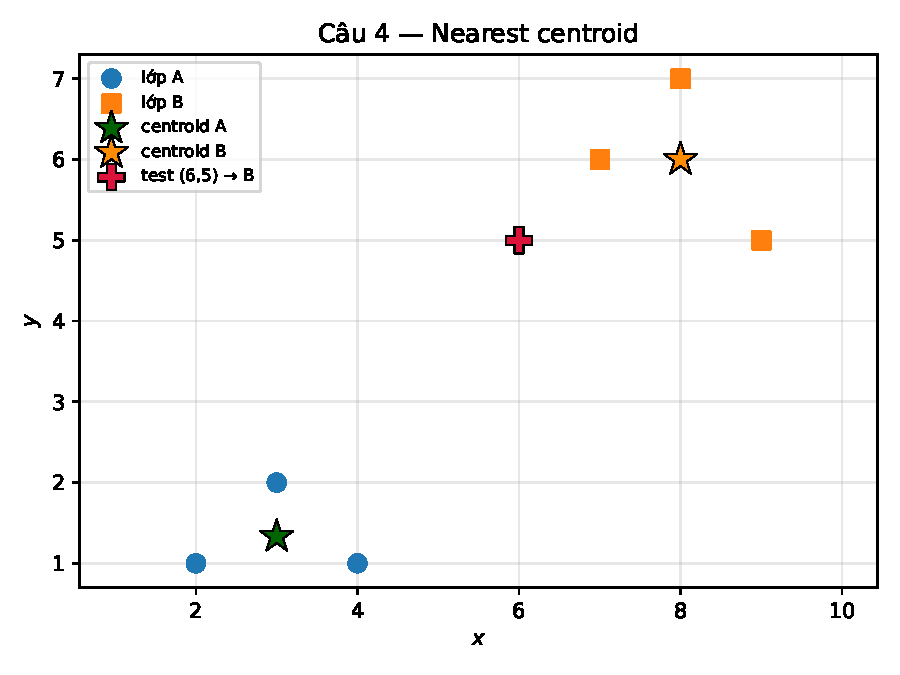
\includegraphics[width=0.72\linewidth]{figures/q4_centroids.pdf}
  \caption{Câu 4: điểm huấn luyện, centroid hai lớp và điểm thử.}
\end{figure}

%--------------------------------------------------------------------
\subsection*{Câu 5. LWR (kernel Gaussian)}

Mô hình \emph{tham chiếu} $h(x)=1+2x$.

\textbf{(1)} $h(2{,}5)=1+2\cdot 2{,}5=6$.

\textbf{(2)} $|x_i-2{,}5|$ lần lượt: $1{,}5$; $0{,}5$; $0{,}5$; $1{,}5$.

\textbf{(3)} Với $\tau=1$: $w_i=\exp\bigl(-(x_i-2{,}5)^2/2\bigr)$:
\[
w\approx(0{,}325;\ 0{,}882;\ 0{,}882;\ 0{,}325).
\]

\textbf{(4) Bổ sung --- hồi quy tuyến tính có trọng số:}
Với thiết kế $[1\,\ x]^\top$ và trọng số $w_i$ ở trên, hệ số WLS tại $x=2{,}5$ cho $y\in\{3,5,7,9\}$ cho \(\hat y(2{,}5)=6\) (trùng $h(2{,}5)$ vì bốn điểm nằm trên cùng đường thẳng $y=1+2x$).

%--------------------------------------------------------------------
\subsection*{Câu 6. COVID symptoms và Hamming}

Mã hóa Yes$=1$, No$=0$. Vector thử $(1,1,1,1,0,0,0,0,0)$.

Bảng Hamming (đã sort): có hai mẫu trùng khớp hoàn toàn (khoảng cách $0$, Positive); tiếp theo $d=2$, $d=3$, $d=4$, $d=5$\,\ldots

\textbf{k-NN đa số:} với $k\in\{1,3,5,7\}$ các láng giềng gần đều cho đa số \textbf{Positive} $\Rightarrow$ dự đoán \textbf{Positive}.

\textbf{Weighted k-NN ($k=3$, $w_i=1/d$, chuẩn hóa):} hai láng giềng $d=0$ (cùng Positive) nhận gần hết trọng số; láng giềng $d=2$ (Negative) có trọng số rất nhỏ. Tổng trọng số thiên \textbf{Positive} $\Rightarrow$ \textbf{Positive}.

%--------------------------------------------------------------------
\subsection*{Phân tích dữ liệu triệu chứng (tập huấn luyện)}

Từ $6$ ca \textbf{Positive} và $4$ ca \textbf{Negative}:

\begin{itemize}\setlength\itemsep{0pt}
  \item \textbf{Xuất hiện nhiều nhất trong Positive:} \textbf{Sốt, Ho khan, Mệt mỏi} đều đạt $6/6$ (bằng nhau, tối đa).
  \item \textbf{Ít nhất trong Positive:} \textbf{Tiêu chảy} ($1/6$). Nếu xét toàn tập, \textbf{Tiêu chảy} cũng có tổng số lần $1$ là nhỏ nhất.
  \item \textbf{Đặc trưng dễ gây nhiễu:} Các triệu chứng hiếm hoặc biến thiên mạnh giữa lớp (\emph{ví dụ} tiêu chảy chỉ gặp ở một ca Positive, hoặc đau ngực chỉ vài ca) có thể làm các mẫu cục bộ ``nhảy lớp'' khi $k$ nhỏ.
  \item \textbf{Phù hợp similarity-based learning:} Mỗi bệnh nhân là vector triệu chứng; bệnh cùng nhóm thường có mẫu gần nhau theo Hamming, nên k-NN/weighted k-NN diễn giải được theo ``các ca tương tự'' --- gần gũi cách ra quyết định lâm sàng tham chiếu hồ sơ tương tự (mang tính minh họa học tập, không thay thế quy trình y tế).
\end{itemize}

%--------------------------------------------------------------------
\subsection*{Câu hỏi tư duy về k-NN}

\begin{enumerate}\setlength\itemsep{2pt}
  \item Với $10^8$ bệnh nhân, k-NN phải tính khoảng tới (gần như) toàn bộ tập khi không có cấu trúc chỉ mục $\Rightarrow$ \textbf{chậm, tốn bộ nhớ}; cần LSH, KD-tree, hoặc chuyển sang mô hình có huấn luyện tham số rút gọn.
  \item \textbf{Lazy learning:} không huấn luyện mô hình tường minh trước; chỉ lưu dữ liệu, khi có truy vấn mới đo khoảng và bỏ phiếu.
  \item \textbf{Nhị phân:} Euclidean trên $\{0,1\}$ coi hai bit khác nhau là ``1 đơn vị trên trục'' nhưng bình phương khác với \emph{đếm lệch bit}; Hamming khớp ngữ nghĩa ``khác bao nhiêu triệu chứng'' và ổn định khi không muốn giả định hình học $\mathbb{R}^d$.
  \item \textbf{Mất cằn bằng lớp:} có ảnh hưởng --- lớp đông dễ chiếm đa số láng giềng; nên cân trọng số theo tần suất lớp, chọn $k$ cẩn thận, hoặc lấy mẫu lại/cân bằng dữ liệu.
\end{enumerate}
